%!TEX TS-program = xelatex
%!TEX encoding = UTF-8 Unicode

\documentclass[12pt]{extarticle}
% extarticle is like article but can handle 8pt, 9pt, 10pt, 11pt, 12pt, 14pt, 17pt, and 20pt text

\def \ititle {Origins of Mind}

\def \isubtitle {Lecture 07}

\def \iauthor {Stephen A. Butterfill}
\def \iemail{s.butterfill@warwick.ac.uk}
\date{}

%for strikethrough
\usepackage[normalem]{ulem}

\input{$HOME/Documents/submissions/preamble_steve_handout}

%\bibpunct{}{}{,}{s}{}{,}  %use superscript TICS style bib
%remove hanging indent for TICS style bib
%TODO doesnt work
\setlength{\bibhang}{0em}
%\setlength{\bibsep}{0.5em}


%itemize bullet should be dash
\renewcommand{\labelitemi}{$-$}

\begin{document}

\begin{multicols}{3}

\setlength\footnotesep{1em}


\bibliographystyle{newapa} %apalike

%\maketitle
%\tableofcontents




%---------------
%--- start paste




\def \ititle {Lecture 07}

\begin{center}

{\Large

\textbf{\ititle}

}



\iemail %

\end{center}



\section{Knowledge of Mind}

\textit{Mindreading} is
the process of
identifying mental states and purposive actions
as the mental states and purposive actions of a particular subject.

‘In saying that an individual has a theory of mind, we mean that the individual imputes mental states to himself and to others’
\citep[p.\ 515]{premack_does_1978}

In a standard \textit{false belief task}, `[t]he subject is aware that he/she and
another person [Maxi] witness a certain state of affairs x. Then, in the absence of
the other person the subject witnesses an unexpected change in the state of affairs
from x to y' \citep[p.\ 106]{Wimmer:1983dz}. The task is designed to measure the
subject's sensitivity to the probability that Maxi will falsely believe x to obtain.

Three-year-olds systematically fail to predict actions \citep{Wimmer:1983dz}
and desires \citep{Astington:1991kk} based on false beliefs; they similarly
fail to retrodict beliefs \citep{Wimmer:1998kx} and to select arguments
suitable for agents with false beliefs \citep{Bartsch:2000es}.
They fail some low-verbal and nonverbal false belief tasks
\citealp{Call:1999co,low:2010_preschoolers,krachun:2009_competitive,krachun:2010_new}; they fail whether the question concerns others' or their own (past)
false beliefs \citep{Gopnik:1991db}; and they fail whether they are
interacting or observing \citep{Chandler:1989qa}.



\section{Infants Track False Beliefs}

One-year-old children predict actions of agents with false beliefs about the
locations of objects \citep{Clements:1994cw,Onishi:2005hm,Southgate:2007js},
and about the contents of containers \citep{he:2011_false}, taking into
account verbal communication \citep{Song:2008qo,scott:2012_verbal_fb}.
They
will also choose ways of helping \citep[]{Buttelmann:2009gy} and
communicating \citep{Knudsen:2011fk,southgate:2010fb} with others depending on
whether their beliefs are true or false. And in much the way that irrelevant
facts about the contents of others’ beliefs modulate adult subjects’ response
times, such facts also affect how long 7-month-old infants look at some
stimuli \citep[]{kovacs_social_2010}.



\section{Mindreading: a Developmental Puzzle}

An \emph{A-Task} is any false belief task that children tend to fail until around
three to five years of age.

\begin{enumerate}
\item Children fail A-tasks
because they rely on a model of minds and actions that does not incorporate beliefs.
\item Children pass non-A-tasks
by relying on a model of minds and actions that does incorporate beliefs.
\item At any time, the child has a single model of minds and actions.
\end{enumerate}

For adults (and children who can do this),
representing perceptions and beliefs as such---and even merely holding in mind
what another believes, where no inference is required---involves a measurable
processing cost \citep{apperly:2008_back,apperly:2010_limits}, consumes attention
and working memory in fully competent adults \citealp{Apperly:2009cc,
lin:2010_reflexively, McKinnon:2007rr},  may require inhibition \citep{bull:2008_role}
and makes demands on executive function \citep{apperly:2004_frontal,samson:2005_seeing}.



\section{Mindreading in Adults: Dual Processes}

Is mindreading automatic?
(More carefully: Does belief tracking in human adults depend only
on processes which are automatic?)

A process is \emph{automatic} to the degree that whether it occurs is independent of its
relevance to the particulars of the subject's task, motives and aims.

There is evidence that some mindreading in human adults is
entirely a consequence of relatively automatic processes
\citep{kovacs_social_2010,Schneider:2011fk,Wel:2013uq}, and
that not all mindreading in human adults is
\citep{apperly:2008_back,apperly_why_2010,Wel:2013uq}.

\citet{qureshi:2010_executive} found that automatic and nonautomatic
mindreading processes are differently influenced by cognitive load, and
\citet{todd:2016_dissociating} provided evidence that adding time pressure
affects nonautomatic but not automatic mindreading processes.

‘Participants never reported belief tracking when questioned in an open format after the experiment (“What do you think this experiment was about?”). Furthermore, this verbal debriefing about the experiment’s purpose never triggered participants to indicate that they followed the actor’s belief state’ \citep[p.~2]{Schneider:2011fk}

\emph{Dual Process Theory of Mindreading}.
Automatic and nonautomatic mindreading processes are independent in
this sense: different conditions influence whether they occur and
which ascriptions they generate \citep[e.g.][]{todd:2016_dissociating,qureshi:2010_executive}.



\section{Minimal Theory of Mind}

An agent’s \emph{field} is a set of objects related to the agent by proximity, orientation and other factors.

First approximation: an agent \emph{encounters} an object just if it is in her field.

A \emph{goal} is an outcome to which one or more actions are, or might be, directed.

%(Not to be confused with a \emph{goal-state}, which is an intention or other state of an agent linking an action to a particular goal to which it is directed.)

\textbf{Principle 1}: one can’t goal-directedly act on an object unless one has encountered it.

Applications: subordinate chimps retrieve food when a dominant is not informed of its
          location \citep{Hare:2001ph}; when observed scrub-jays prefer to cache in shady, distant and
          occluded locations \citep{Dally:2004xf,Clayton:2007fh}.

First approximation: an agent \emph{registers} an object at a location just if she most recently encountered the object at that location.

A registration is \emph{correct} just if the object is at the location it is registered at.

\textbf{Principle 2}: correct registration is a condition of successful action.

Applications: 12-month-olds point to inform depending on their informants’ goals and ignorance \citep{Liszkowski:2008al};
          chimps retrieve food when a dominant is misinformed about its location \citep{Hare:2001ph};
          scrub-jays observed caching food by a competitor later re-cache in private \citep{Clayton:2007fh,Emery:2007ze}.

\textbf{Principle 3}: when an agent performs a goal-directed action and the goal specifies an object, the agent will act as if the object were actually in the location she registers it at.

Applications: some false belief tasks \citep{Onishi:2005hm,Southgate:2007js,Buttelmann:2009gy}.



\section{Signature Limits}

Automatic belief-tracking in adults and
belief-tracking in infants are both subject to signature limits
associated with minimal theory of mind
(\citealp{wang:2015_limits,Low:2012_identity,low:2014_quack,mozuraitis:2015_privileged};
contrast \citealp{scott:2015_infants}).

\begin{center}

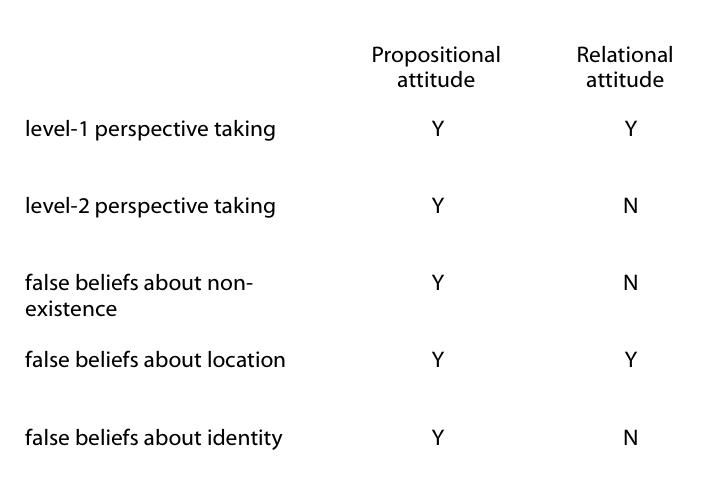
\includegraphics[width=0.25\textwidth]{fig/signature_limits_table.png}

\end{center}

\begin{center}

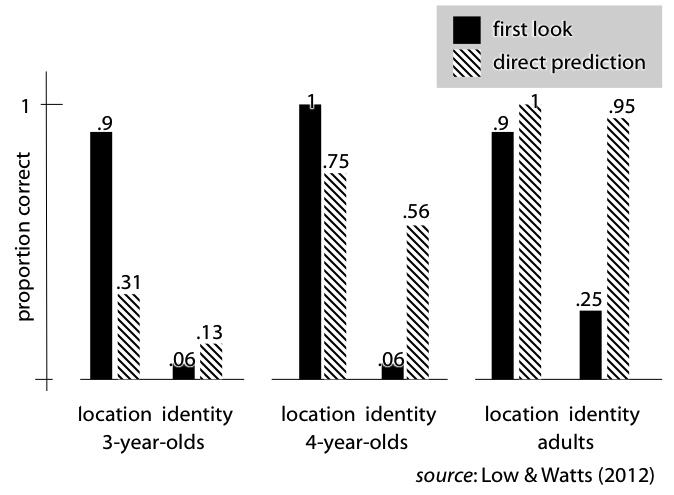
\includegraphics[width=0.3\textwidth]{fig/low_2012_fig.png}

\end{center}

Objection:
‘the theoretical arguments offered [...] are [...] unconvincing, and [...]
the data can be explained in other terms’
(\citealp{carruthers:2015_two}; see also \citealp{carruthers:2015_mindreading}).


    



%--- end paste
%---------------

\footnotesize
\bibliography{$HOME/endnote/phd_biblio}

\end{multicols}

\end{document}
